\section{Exercise 8.14: Smoothing a newspaper picture}

The script \texttt{smooth\_picture.m} reads \texttt{van\_aartsen.jpg} into a matrix $f$ of $M = 894$ rows by $N = 1192$ columns (grey values from $48$ to $255$) and computes its spectrum $F$ with \texttt{fft2}. The second matrix $g$ has the same size, with $g[m,n] = 1$ for $0 \le m, n \le L-1$ (the top-left $L \times L$ pixels) and $g[m,n] = 0$ elsewhere; initially $L = 5$. The spectra $F$, $G$ and their pointwise product $FG$ are computed, and the convolution follows from the convolution property (8.21):
\[
f ** g = \mathrm{IDFT2}\{F\,G\}.
\]
Below, $k_x$ and $k_y$ denote the DFT indices along $x$ (columns) and $y$ (rows), counted from the centre after \texttt{fftshift}; index $k_x$ corresponds to a pattern that repeats $k_x$ times across the width of the picture, i.e.\ with a period of $N/k_x$ pixels.

\subsection*{The spectrum $FG$}

The values of $F$ and $FG$ span many orders of magnitude: the term at $k_x = k_y = 0$ alone equals the sum of all grey values. Plotted on a linear colour scale, almost the whole spectrum would therefore be black. \Cref{fig:smooth-spectra} shows $\log(1 + |F|)$ and $\log(1 + |FG|)$ instead, after \texttt{fftshift}, so that $k_x = k_y = 0$ lies in the centre.

\begin{figure}[H]
    \centering
    \begin{subfigure}{0.49\linewidth}
        \centering
        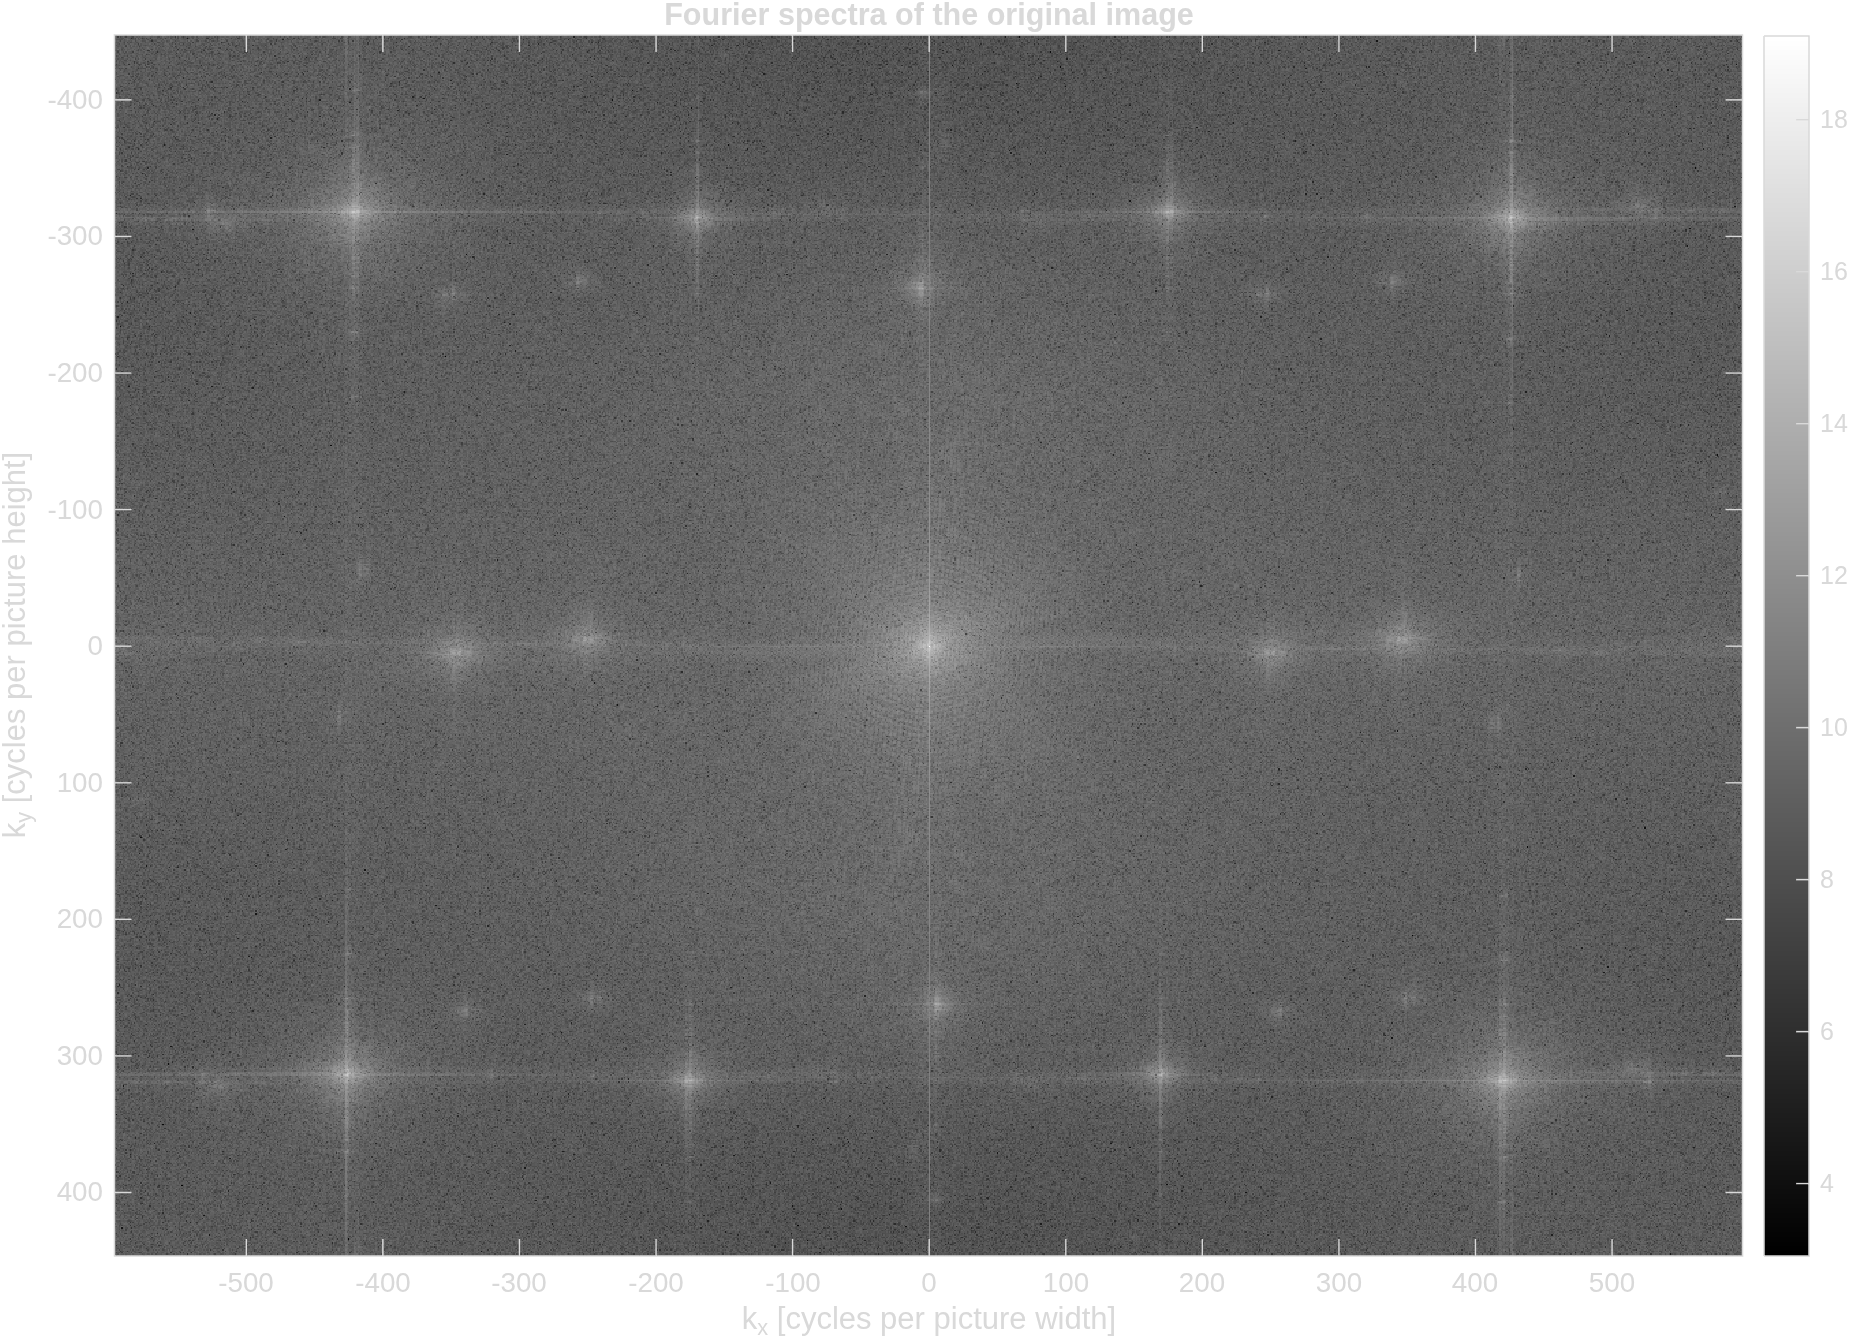
\includegraphics[width=\linewidth]{Figures/smoothing_F_log.png}
        \caption{$\log(1 + |F|)$, original picture}
    \end{subfigure}
    \hfill
    \begin{subfigure}{0.49\linewidth}
        \centering
        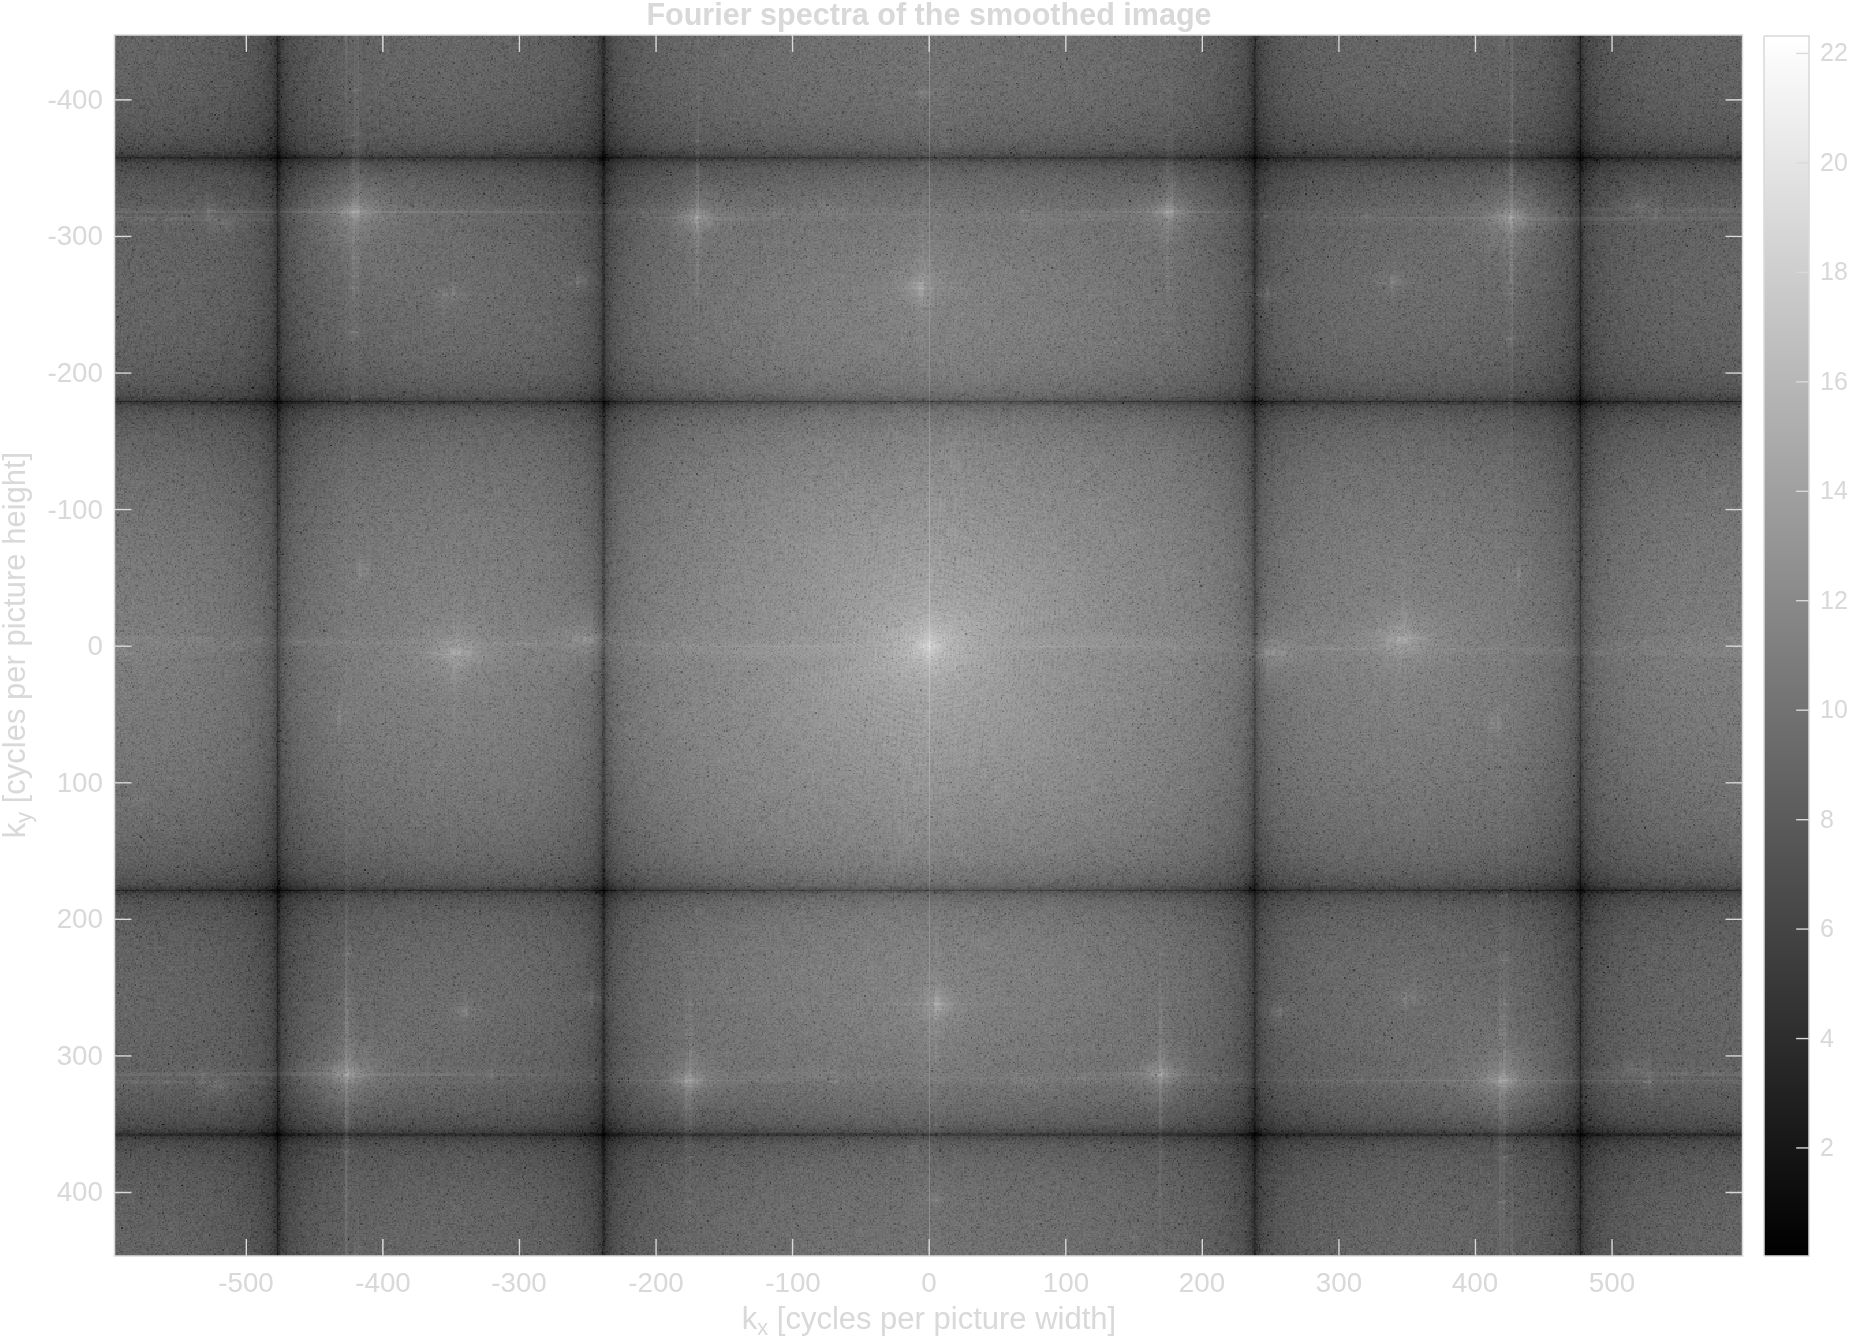
\includegraphics[width=\linewidth]{Figures/smoothing_FG_log.png}
        \caption{$\log(1 + |FG|)$, smoothed with $L = 5$}
    \end{subfigure}
    \caption{Spectra of the original and the smoothed picture after \texttt{fftshift}. The axes give the DFT indices $k_x$ and $k_y$, in cycles per picture width and height.}
    \label{fig:smooth-spectra}
\end{figure}

\textbf{Spectrum of the original.} The bright centre contains the low spatial frequencies: the large, slowly varying shapes of the face and background. Away from the centre, $|F|$ shows a regular lattice of isolated peaks. These come from the halftone raster of the newspaper print, the regular grid of small ink dots with which a newspaper prints a photo: a periodic pattern gives sharp peaks at its spatial frequency and its multiples. The strongest peaks lie at $(k_x, k_y) = (\pm 426, \pm 314)$ and $(\pm 422, \mp 318)$, which corresponds to a period of $N/426 \approx 2.8$ pixels in $x$ and $M/314 \approx 2.8$ pixels in $y$.

\textbf{Spectrum of $g$.} Evaluating the DFT of the $L \times L$ block gives two geometric sums, with magnitude
\[
|G[k_x, k_y]| = \left| \frac{\sin(\pi k_x L / N)}{\sin(\pi k_x / N)} \right| \cdot \left| \frac{\sin(\pi k_y L / M)}{\sin(\pi k_y / M)} \right|,
\]
the discrete counterpart of the sinc function that is the Fourier transform of a rectangle. Its maximum is $G[0,0] = L^2 = 25$. It vanishes when $k_x L / N$ or $k_y L / M$ is a non-zero integer, i.e.\ for patterns that fit a whole number of times into the $L \times L$ block, so that they average out. For $L = 5$ this happens at $k_x = p\,N/L = 238.4\,p$ and $k_y = p\,M/L = 178.8\,p$ ($p = \pm 1, \pm 2, \dots$). Since these values are not integers, $|G|$ has deep minima rather than exact zeros: the first minimum along $x$ lies at $k_x = 238$, where $|G| = 0.045$, compared with $25$ at the centre. The first minimum along $y$ lies at $k_y = 179$.

\textbf{Spectrum of $FG$.} Multiplying by $G$ produces the dark vertical lines in \cref{fig:smooth-spectra} at $k_x \approx \pm 238$ and $\pm 477$ and the dark horizontal lines at $k_y \approx \pm 179$ and $\pm 358$. The centre is kept, while the higher frequencies are damped: $g$ acts as a low-pass filter. The raster peaks are still visible in $\log(1 + |FG|)$, but they are strongly reduced. At the strongest raster peaks $|G| / G[0,0] = 0.021$, so relative to the mean brightness they are suppressed by a factor of about $48$. On the logarithmic colour scale this is only a shift of $\ln(0.021) \approx -3.9$, which is why they do not disappear from the plot.

\subsection*{Original and smoothed picture; relation to exercise 8.2}

\Cref{fig:smooth-compare} shows the original and the smoothed picture ($L = 5$) side by side. The raster of the newspaper print, clearly visible in the original, has disappeared. Features much larger than the $5 \times 5$ block, such as the glasses, the eyes and the outline of the face, remain recognisable and are only slightly softened.

\begin{figure}[H]
    \centering
    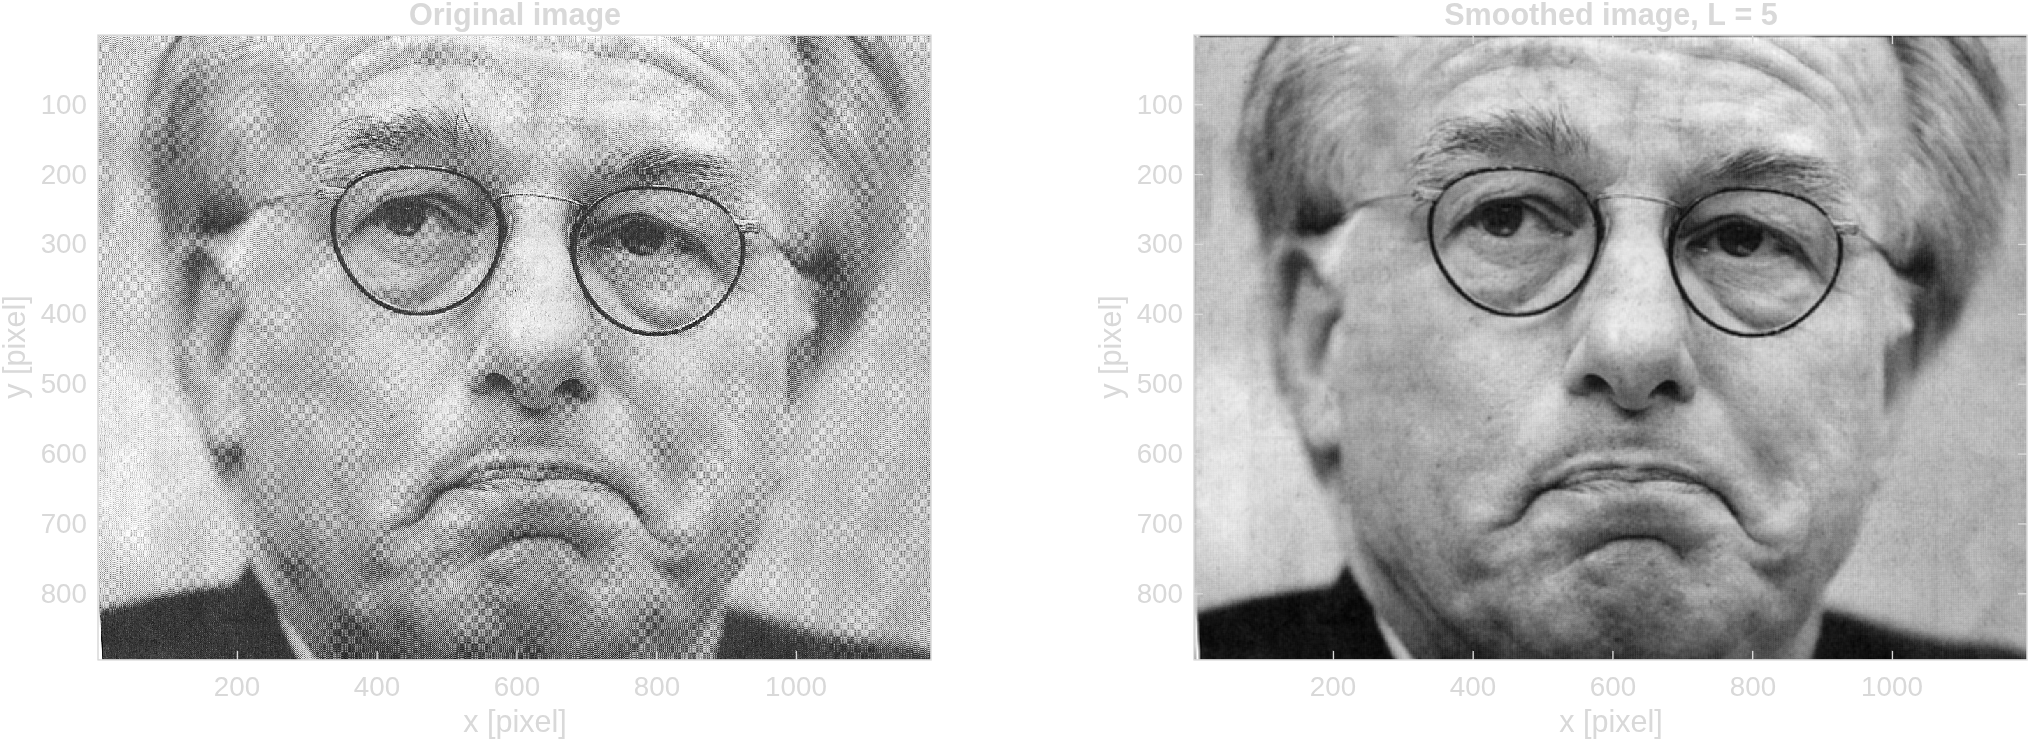
\includegraphics[width=\linewidth]{Figures/smoothing_original_vs_smoothed.png}
    \caption{Original picture (left) and the picture smoothed with $L = 5$ (right), computed with the convolution property (8.21).}
    \label{fig:smooth-compare}
\end{figure}

Writing out the inverse DFT of $FG$ gives the circular convolution
\[
(f ** g)[m, n] = \sum_{i=0}^{L-1} \sum_{j=0}^{L-1} f\big[(m - i) \bmod M,\; (n - j) \bmod N\big].
\]
Each pixel of the result is therefore the unweighted sum of the $L \times L$ square of pixels whose bottom-right corner is pixel $(m, n)$. As a check, the result at MATLAB pixel $(400, 600)$ is $5962$, exactly the sum of \texttt{f(396:400, 596:600)}.

This is the discrete version of exercise 8.2, where $g(x, y) = \frac{1}{ab} \operatorname{rect}(x/a) \operatorname{rect}(y/b)$ makes $f ** g$ the unweighted average of $f$ over a rectangle centred on $(x, y)$. There are three differences.
\begin{enumerate}
    \item \textbf{Normalisation.} The $g$ of exercise 8.2 has unit integral, while ours sums to $L^2$ (equivalently $G[0,0] = L^2$). The result is the sum over the square, $L^2$ times the average: for $L = 5$ the smoothed values range from $2078$ to $6371$, against $48$ to $255$ in the original (ratio of the maxima $24.98$). This is invisible in \cref{fig:smooth-compare} because \texttt{imagesc} rescales the colour map. Dividing $g$ by $L^2$ gives exactly the average of exercise 8.2.
    \item \textbf{Position of the square.} The square is not centred on the pixel but has it as its bottom-right corner. The smoothed picture is therefore shifted by $(L-1)/2$ pixels down and to the right: $2$ pixels for $L = 5$, not visible, but $49.5$ pixels for $L = 100$. A centred average would require the block of ones to be centred on $g[0,0]$, wrapping around the edges of $g$.
    \item \textbf{Edges.} The DFT treats the picture as one period of a pattern that repeats in both directions. Squares near the top and left edges therefore take pixels from the bottom and right edges of the picture, instead of the zeros or missing values of an ordinary convolution.
\end{enumerate}

As a check of the convolution property, the script also computes the ordinary (non-circular) convolution directly with \texttt{conv2(f, ones(L))}, keeping its first $M \times N$ values so that the square has the same position. Away from the top $L-1$ rows and the left $L-1$ columns, where no wrap-around occurs, both results agree to within $1.3 \cdot 10^{-11}$, i.e.\ up to rounding. Along the top row they differ by up to $5.1 \cdot 10^{3}$, which is the wrap-around of item 3.

\subsection*{Influence of $L$}

\Cref{fig:smooth-L} shows the result for $L = 1$, $10$ and $100$.

\begin{figure}[H]
    \centering
    \begin{subfigure}{0.32\linewidth}
        \centering
        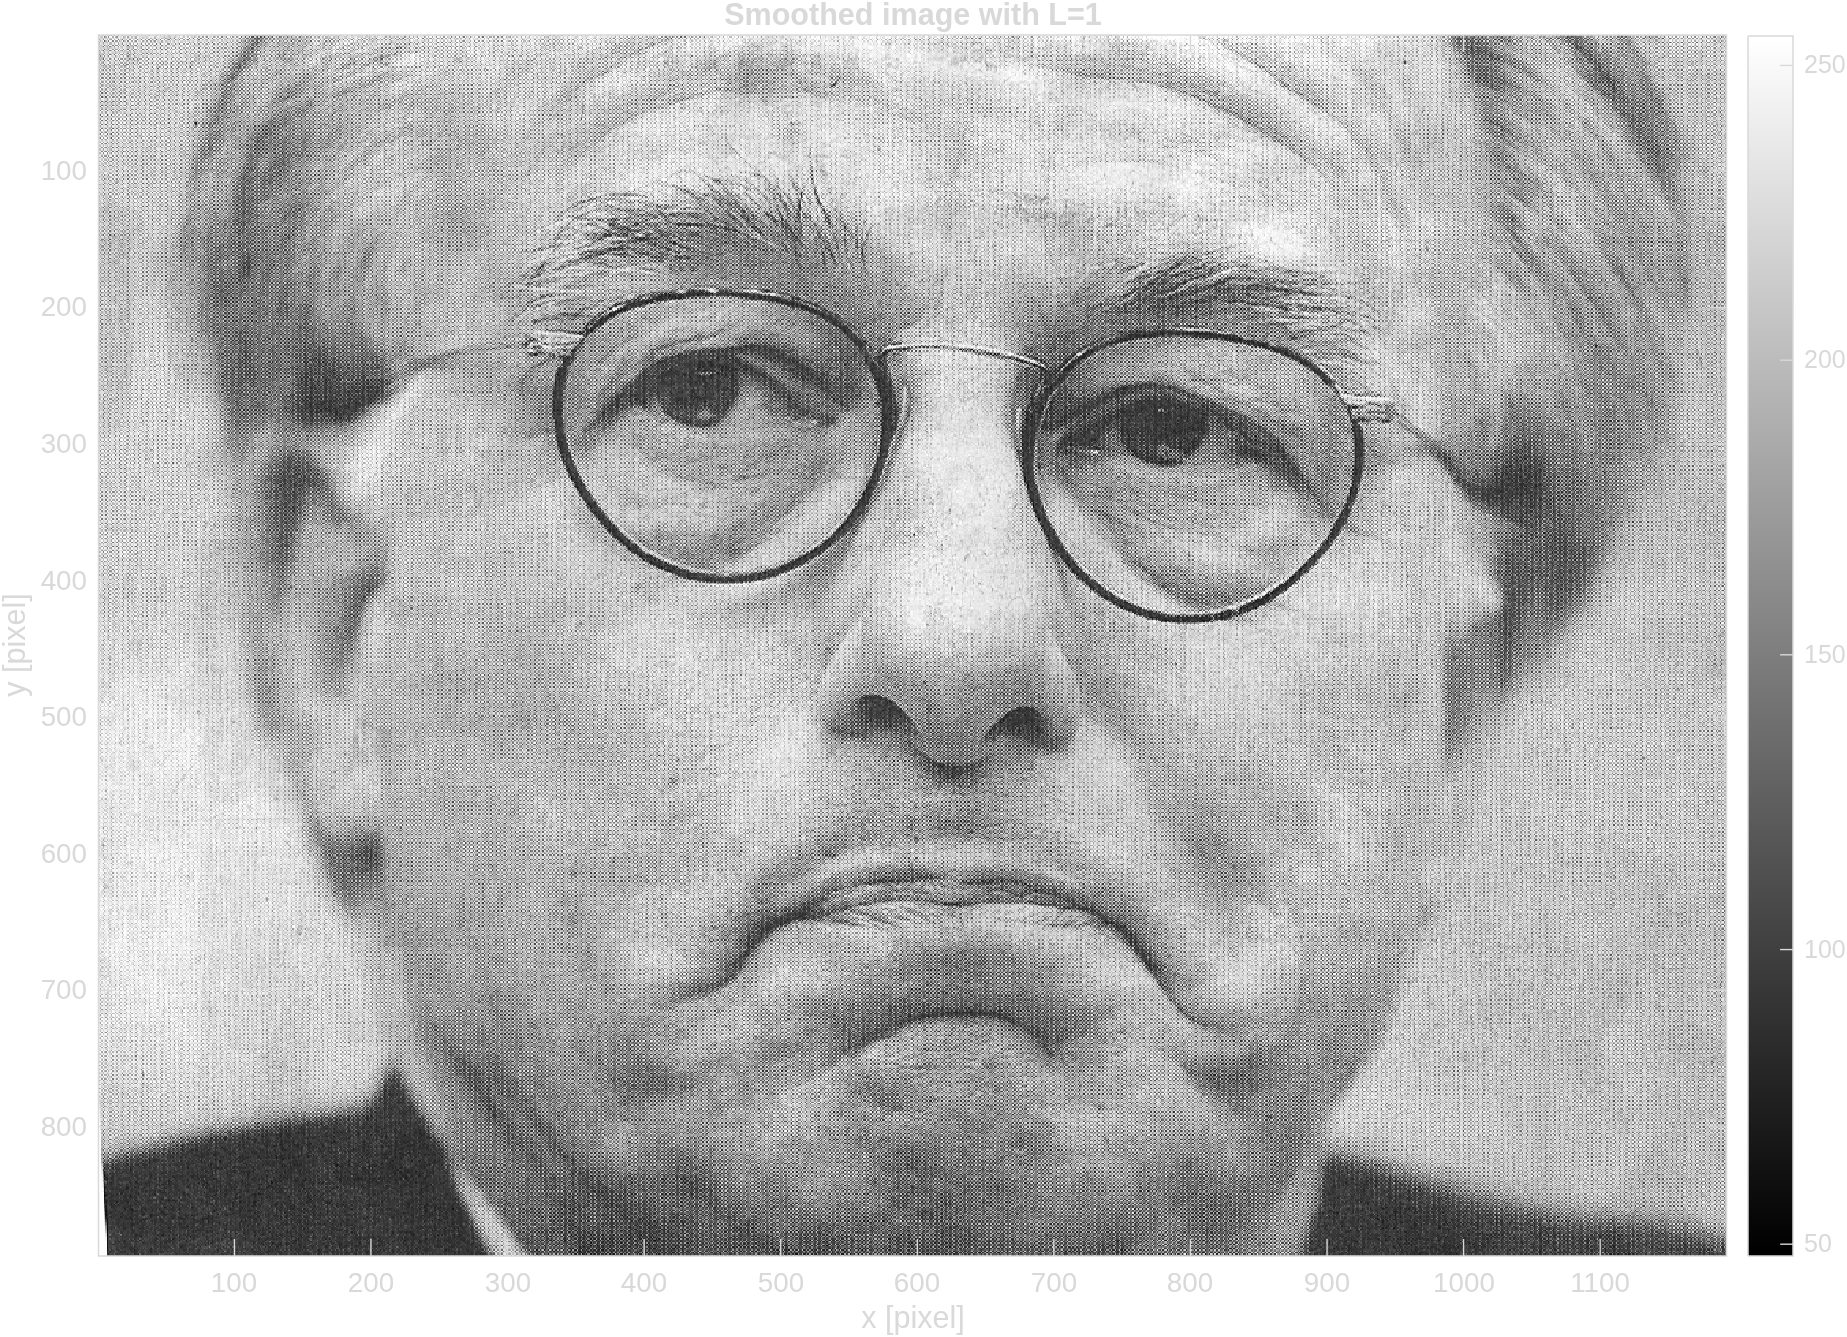
\includegraphics[width=\linewidth]{Figures/smoothing_f_convolution_L1.png}
        \caption{$L = 1$}
    \end{subfigure}
    \hfill
    \begin{subfigure}{0.32\linewidth}
        \centering
        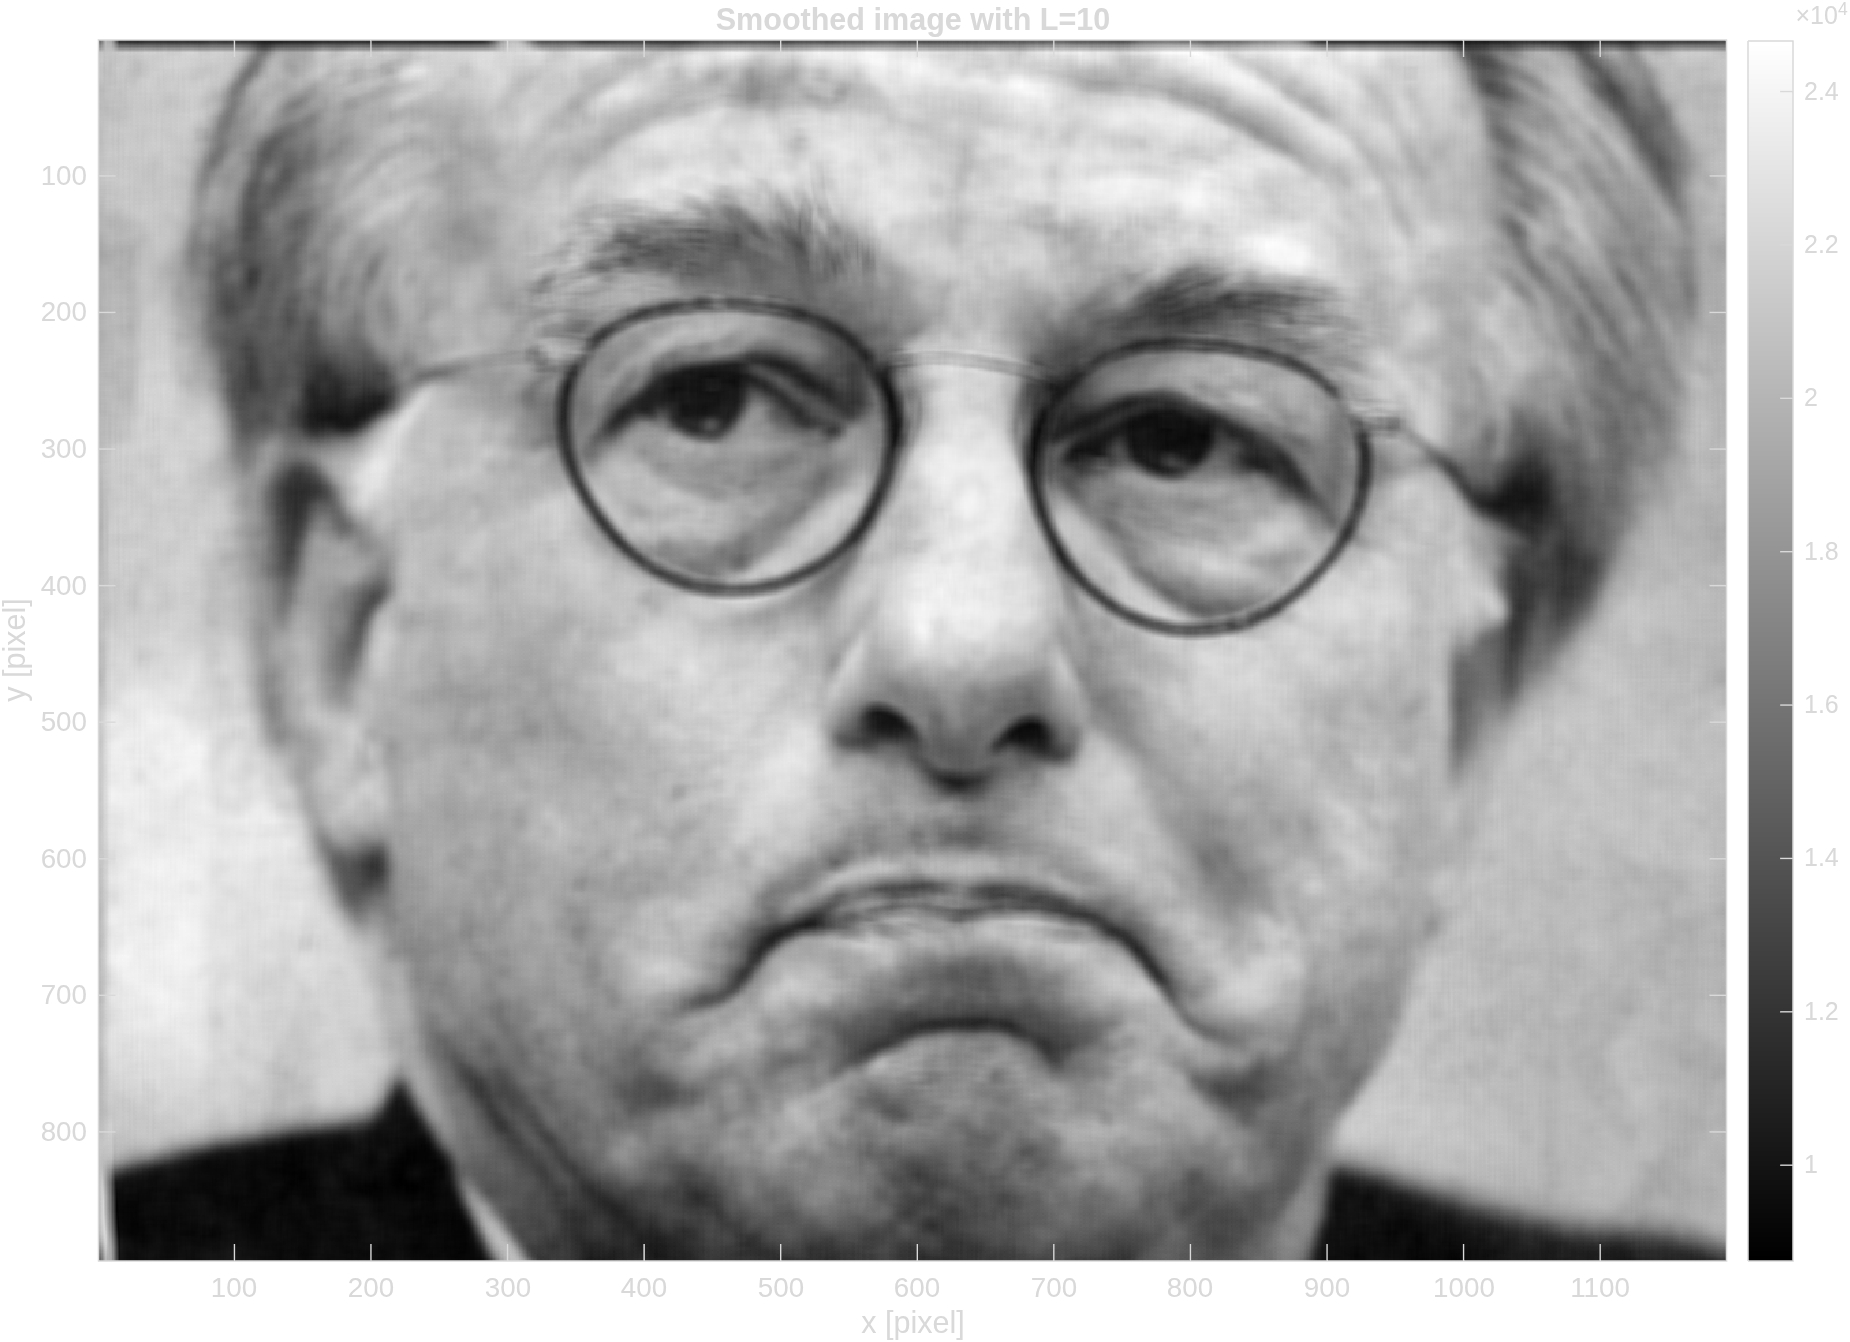
\includegraphics[width=\linewidth]{Figures/smoothing_f_convolution_L10.png}
        \caption{$L = 10$}
    \end{subfigure}
    \hfill
    \begin{subfigure}{0.32\linewidth}
        \centering
        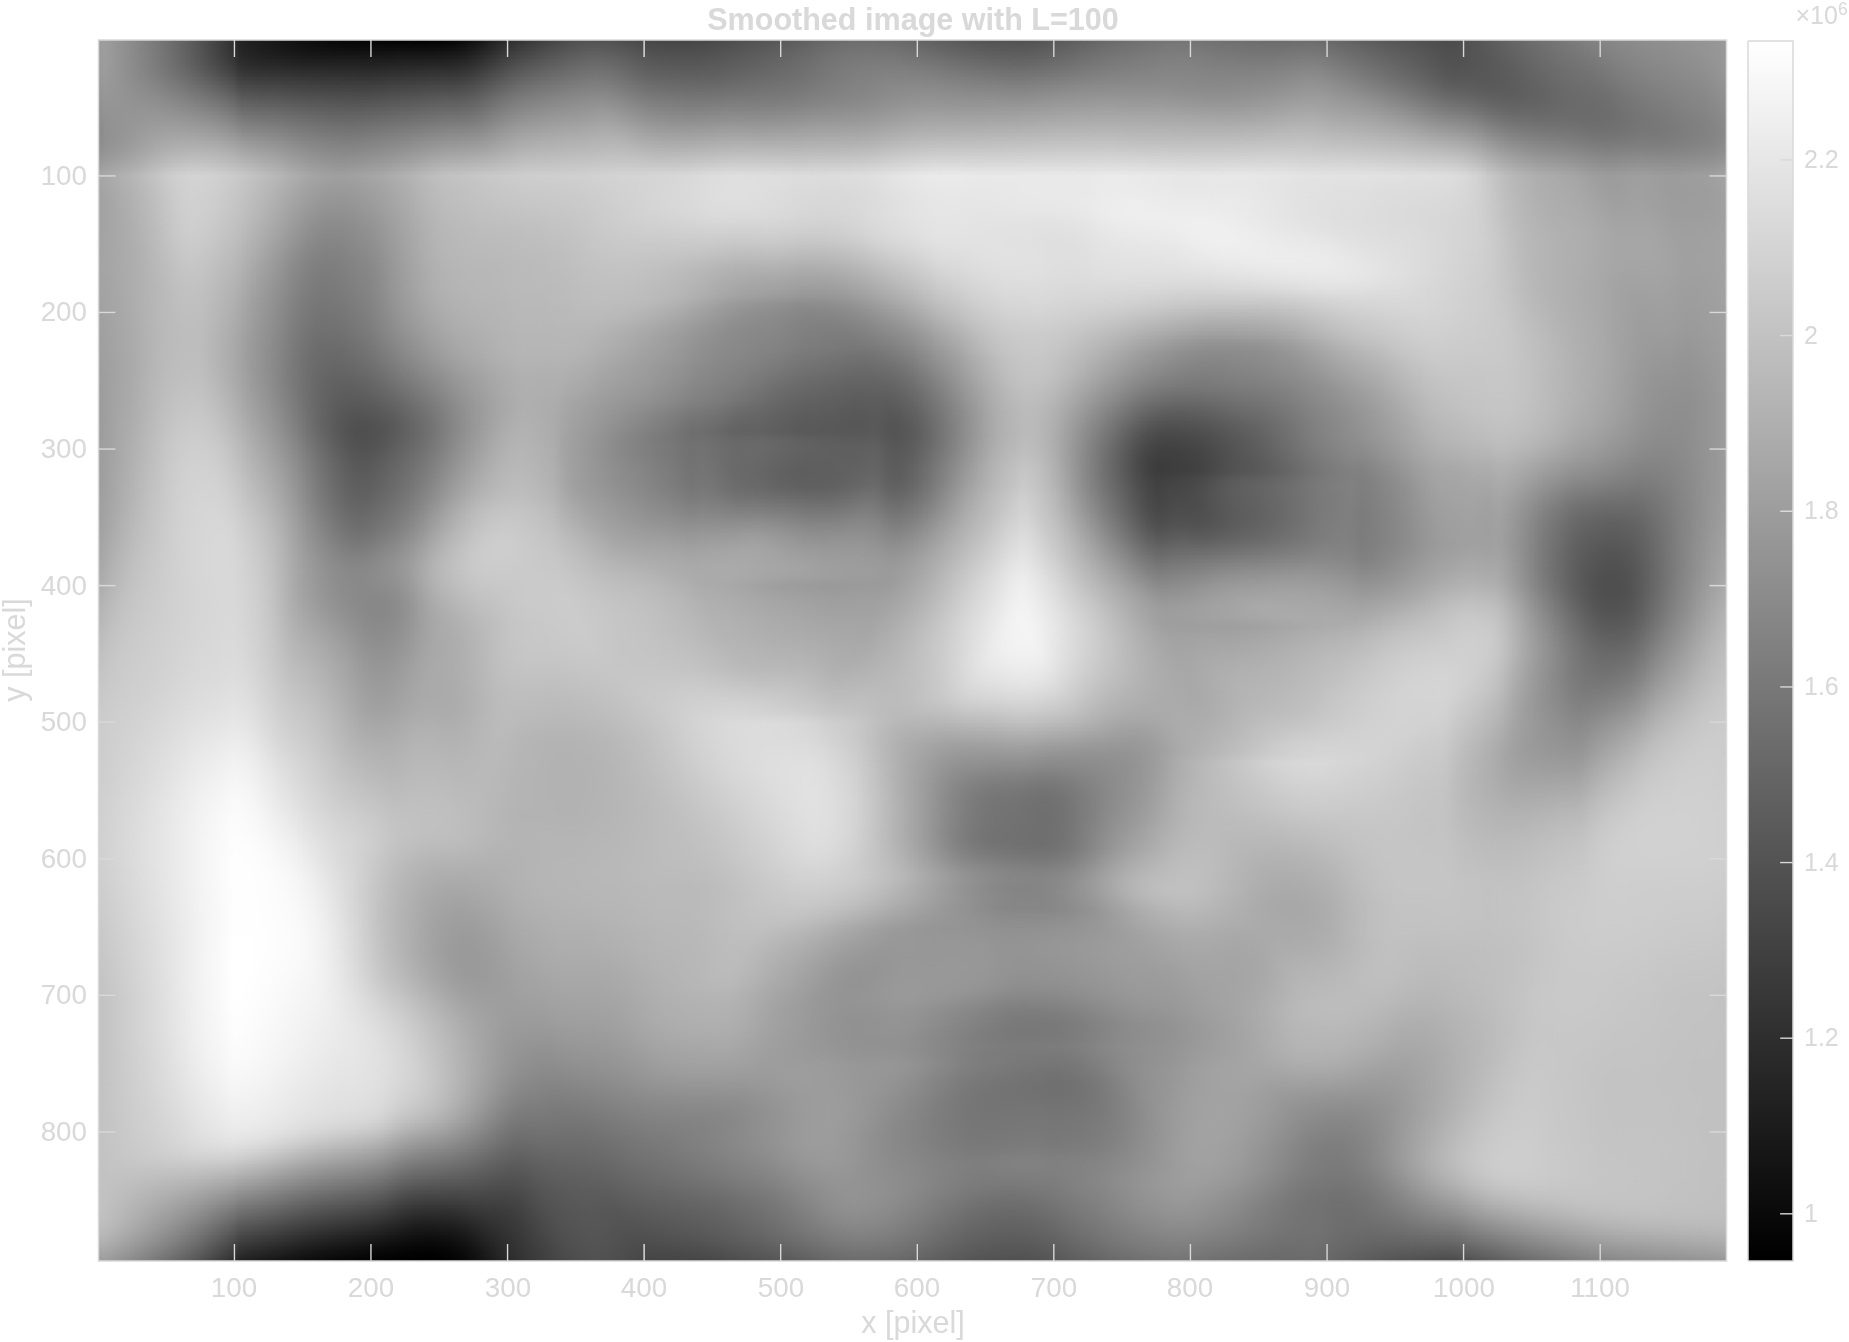
\includegraphics[width=\linewidth]{Figures/smoothing_f_convolution_L100.png}
        \caption{$L = 100$}
    \end{subfigure}
    \caption{The picture convolved with an $L \times L$ block of ones for three values of $L$.}
    \label{fig:smooth-L}
\end{figure}

The minima of $|G|$ lie at $k_x = p\,N/L$ and $k_y = p\,M/L$, so the central region that $G$ passes shrinks in proportion to $1/L$.
\begin{itemize}
    \item \textbf{Larger $L$.} Fewer frequencies pass and the picture becomes blurrier. For $L = 10$ the first minima move to $k_x \approx \pm 119$ and $k_y \approx \pm 89$, twice as close to the centre as for $L = 5$, and the strongest raster peaks are reduced to $|G|/G[0,0] = 0.012$. The raster is gone, but fine detail such as the texture of the skin is softened as well. For $L = 100$ only the coarse shapes remain, and two artefacts of the method become visible. First, the picture is shifted by about $50$ pixels. Second, there is a dark band along the top edge, caused by the periodic continuation: the squares along the top edge average over the bottom rows of the picture, where the dark jacket is. The mean grey value of the top $20$ rows of the smoothed picture (divided by $L^2$) is $145.4$, against $200.7$ for rows $150$ to $170$. In the original, the mean of the top $20$ rows is $213.1$ and that of the bottom $100$ rows is $140.8$.
    \item \textbf{Smaller $L$.} More high frequencies pass. More detail is preserved, but less of the raster is removed.
    \item \textbf{$L = 1$.} Now $g$ is a single $1$ at $g[0,0]$, a discrete delta peak, so $f ** g = f$ by the discrete form of relation (8.5). Equivalently, $G = 1$ for all $(k_x, k_y)$ and $FG = F$. The computed result equals the original up to rounding: $\max |f ** g - f| = 6.8 \cdot 10^{-13}$.
\end{itemize}

The choice of $L$ is a trade-off between removing the raster and keeping the detail. $L = 5$ spans almost two raster periods ($5 / 2.8 \approx 1.8$), which suppresses the raster by a factor of about $50$ while features much larger than $5$ pixels are preserved.
